\documentclass{beamer}

\usepackage{fancyvrb,tikz, dsfont}

\usetikzlibrary{automata,arrows}

\usetheme{Dresden}

\mode<presentation>

\title{Tolkienizer}
\author{Sean Anderson \and Samuel C. Payson \and Akanksha Vyas}

\begin{document}

\begin{frame}
\titlepage
\end{frame}

\begin{frame}
   \frametitle{Contents}
   \tableofcontents[pausesections]
\end{frame}

\section{Introduction}

\subsection{Introduction to the Problem}

\begin{frame}
   \frametitle{What is Natural Language Processing?}
   \begin{itemize}
      \item Study of human language using AI techniques
      \item Often uses statistical machine learning techniques
      \item Subfields include:
      \begin{itemize}
         \item Morphology
         \item Parsing
         \item Natural Language Understanding
      \end{itemize}
   \end{itemize}
\end{frame}

\begin{frame}
   \frametitle{What is Tolkienizer?}
   \begin{itemize}
      \item Task: generate ``real sounding'' words for a language
      \item Similar to morphology - identifying patterns to learn
      characteristic features of a language
      \item Example: create new ``Elvish sounding'' words from samples of Tolkien's Elvish
      \item Implementation: Hidden Markov Models
   \end{itemize}
\end{frame}

\section{Who Is This Markov, and Why Does He Hide His Models?}

\subsection{Markov Processes and Hidden Markov Models}

\begin{frame}
   \frametitle{What is a Markov Process?}
   \begin{enumerate}
   \item[] <2-> \small{\textbf{Markov Process:} A \textcolor{red}{stochastic} process with
   the \textcolor{red}{Markov property}.}
   \item[] <3-> \textbf{Stochastic Process:} A random process parametrized by time.
   \item[] <4-> \textbf{Markov Property:} Memoryless!
   \item[] <3->
   \begin{columns}[c]
   \column{1.5in} 
   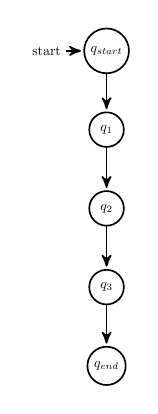
\begin{tikzpicture} [scale=0.5,->,>=stealth',shorten >=1pt,%
   auto,node distance=2cm,semithick,transform shape]

   \node[state,initial]  (q0)               {$q_{start}$};
   \node[state]          (q1) [below of=q0] {$q_1$};
   \node[state]          (q2) [below of=q1] {$q_2$};
   \node[state]          (q3) [below of=q2] {$q_3$};
   \node[state]          (q4) [below of=q3] {$q_{end}$};

   \path[->]    (q0) edge               node {}      (q1)
                (q1) edge               node {}      (q2)
                (q2) edge               node {}      (q3)
                (q3) edge               node {}      (q4);
   \end{tikzpicture}
   \column{1.5in} 
   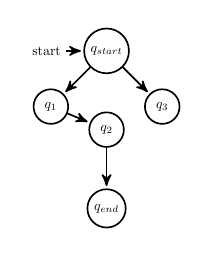
\begin{tikzpicture} [scale=0.5,->,>=stealth',shorten >=1pt,%
   auto,node distance=2cm,semithick,transform shape]

   \node[state,initial]  (q0)                        {$q_{start}$};
   \node[state]          (q1) [below left of=q0]     {$q_1$};
   \node[state]          (q2) [below of=q0]          {$q_2$};
   \node[state]          (q3) [below right of=q0]    {$q_3$};
   \node[state]          (q4) [below of=q2]          {$q_{end}$};

   \path[->]    (q0) edge               node {}      (q1)
                (q1) edge               node {}      (q2)
                (q0) edge               node {}      (q3)
                (q2) edge               node {}      (q4);
   \end{tikzpicture}
   \begin{itemize}
\item[] $\mathds{P} = [q_{end}|q_2,q_1,q_{start}]$
\item[] <6-> $\mathds{P} = [q_{end}|q_2]$
   \end{itemize}
\end{columns}
\end{enumerate} 
\end{frame}

\begin{frame}
   \frametitle{What are Hidden Markov Models's?}
   \begin{enumerate}
   \pause
   \item[] \small{\textbf{Bayesian Networks:} Directed acyclic graphs that
   represent dependencies between variables in a probabilistic model.}
   \pause
   \item[] \small{\textbf{Hidden Markov Models (HMM's):} Bayesion network that
   operates under the assumption that the system to be modeled is a Markov
   Process with hidden states. However, some information about this model is
   revealed. The goal is to guess the model based on that information.}
   \end{enumerate}
\end{frame}

\subsection{How this Applies to our Project}
\begin{frame}
   \frametitle{Why did we need all this?}
   \begin{columns}[c]
      \column{1.5in}
      \begin{center}
         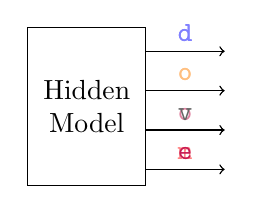
\begin{tikzpicture}
            \path[use as bounding box] (0,0) rectangle (2.5,2);
            \path[draw=black]    <1-> (0,0) rectangle node[text centered,text width=1.5cm] {Hidden Model}(1.5,2);
            \path[draw=black,->] <2-5> (1.5,1.7) -- node[above,blue!50]   {\texttt{d}} (2.5,1.7);
            \path[draw=black,->] <3-5> (1.5,1.2) -- node[above,orange!50] {\texttt{o}} (2.5,1.2);
            \path[draw=black,->] <4-5> (1.5,0.7) -- node[above,purple!50] {\texttt{o}} (2.5,0.7);
            \path[draw=black,->] <5-5> (1.5,0.2) -- node[above,red!50]    {\texttt{m}} (2.5,0.2);

            \path[draw=black,->] <7->  (1.5,1.7) -- node[above,blue!50]   {\texttt{d}} (2.5,1.7);
            \path[draw=black,->] <8->  (1.5,1.2) -- node[above,orange!50] {\texttt{o}} (2.5,1.2);
            \path[draw=black,->] <9->  (1.5,0.7) -- node[above,black!60]   {\texttt{v}} (2.5,0.7);
            \path[draw=black,->] <10-> (1.5,0.2) -- node[above,purple!90]    {\texttt{e}} (2.5,0.2);
         \end{tikzpicture}
      \end{center}
      \column{1.5in}
      \begin{center}
         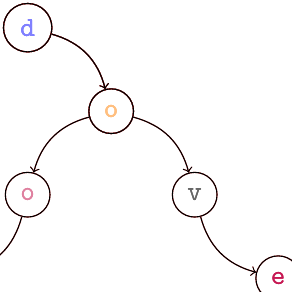
\begin{tikzpicture}[bend angle=30,node distance=1.5cm]
            \path[use as bounding box] (0,0) rectangle (3,-3);
            \path[draw=black] <2> (0,0) node[circle,blue!50,draw=red!70]   (d)  {\texttt{d}};
            \path[draw=black] <3-6> (0,0) node[circle,blue!50,draw=black]   (d)  {\texttt{d}};
            \path[draw=black] <3> node[circle,orange!50,draw=red!70,below right of=d] (o1) {\texttt{o}};
            \path[draw=black] <4-7> node[circle,orange!50,draw=black,below right of=d] (o1) {\texttt{o}};
            \path[draw=black] <3> (d) edge[->,bend left,red!70] (o1);
            \path[draw=black] <4-7> (d) edge[->,bend left] (o1);
            \path[draw=black] <4> node[circle,purple!50,draw=red!70,below left of=o1] (o2) {\texttt{o}};
            \path[draw=black] <5-> node[circle,purple!50,draw=black,below left of=o1] (o2) {\texttt{o}};
            \path[draw=black] <4> (o1) edge[->,bend right,red!70] (o2);
            \path[draw=black] <5-> (o1) edge[->,bend right] (o2);
            \path[draw=black] <5-> node[circle,red!50,draw=red!70,below left of=o2] (m) {\texttt{m}};
            \path[draw=black] <5-> (o2) edge[->,bend left,red!70] (m);
            \path[draw=black] <6-> node[circle,red!50,draw=black,below left of=o2] (m) {\texttt{m}};
            \path[draw=black] <6-> (o2) edge[->,bend left] (m);

            \path[draw=black] <7> (0,0) node[circle,blue!50,draw=red!70]   (d)  {\texttt{d}};
            \path[draw=black] <8-> (0,0) node[circle,blue!50,draw=black]   (d)  {\texttt{d}};

            \path[draw=black] <8> node[circle,orange!50,draw=red!70,below right of=d] (o1) {\texttt{o}};
            \path[draw=black] <9-> node[circle,orange!50,draw=black,below right of=d] (o1) {\texttt{o}};
            \path[draw=black] <8> (d) edge[->,bend left,red!70] (o1);
            \path[draw=black] <9-> (d) edge[->,bend left] (o1);

            \path[draw=black] <9> node[circle,black!60,draw=red!70,below right of=o1] (v) {\texttt{v}};
            \path[draw=black] <9> (o1) edge[->,bend left,red!70] (v);
            \path[draw=black] <10-> node[circle,black!60,draw=black,below right of=o1] (v) {\texttt{v}};
            \path[draw=black] <10-> (o1) edge[->,bend left] (v);

            \path[draw=black] <10> node[circle,purple!90,draw=red!70,below right of=v] (e) {\texttt{e}};
            \path[draw=black] <10> (v) edge[->,bend right,red!70] (e);
            \path[draw=black] <11-> node[circle,purple!90,draw=black,below right of=v] (e) {\texttt{e}};
            \path[draw=black] <11-> (v) edge[->,bend right] (e);
         \end{tikzpicture}
      \end{center}
   \end{columns}
\end{frame}

\section{Development Process}

\subsection{Program Design}
\begin{frame}
   \frametitle{Overall Design}
   \begin{itemize}
      \item Two step process
      \begin{enumerate}
         \item Learn from a large set of words from some language
         \item Produce words that ``seem'' like they are in the language
      \end{enumerate}
      \item In the first phase we construct our Markov Model
      \item In the second we simply let it run.
   \end{itemize}
\end{frame}

\begin{frame}
   \frametitle{Interpreting the Input}
   \begin{itemize}
      \item Lexical Analyzer
      \begin{itemize}
         \item responsible for breaking the input into \emph{tokens}
         \item very flexible, can break up at word or letter boundaries
      \end{itemize}
      \item All tokens are eventually turned into strings
      \item Rest of program designed to deal with strings
      \begin{itemize}
         \item Completely agnostic about the type of the tokens
         \item Any type can be converted to a string
      \end{itemize}
   \end{itemize}
\end{frame}

\begin{frame}
   \frametitle{Representing Markov Models}
   \begin{itemize}
      \item Each state is defined by a sequence of three tokens
      \item The state has a set of tokens, each with a probability of being the
      next token
      \item During the learning phase, watch the input and update probabilites
      according to training data
      \item During the generation phase, follow the Markov Model, emitting
      symbols based on the probabilities at each state
   \end{itemize}
\end{frame}

\subsection{Implementation}

\begin{frame}
   \frametitle{Programming in Go}
   \begin{itemize}
      \item Go offers lightweight threads | hundreds of thousands of concurrent
      processes with minimal overhead.
      \item Efficient communication between lightweight threads, allowing
      programs to be build like UNIX tools (pipe and filter).
      \item Nodes of markov model implemented as individual threads
   \end{itemize}
\end{frame}

\begin{frame}
   \frametitle{Advantages of this Design}
   \begin{itemize}
      \item A single function is easy to implement and maintain.
      \item Nodes know only about themselves, no need for ``glue'' to hold
      software components together.
   \end{itemize}
\end{frame}

\end{document}
